\pdfoutput=1
\documentclass[11pt,a4paper]{article}
\usepackage[utf8]{inputenc}
\usepackage[T1]{fontenc}
\usepackage{lmodern}
\usepackage{amsmath,amssymb}
\usepackage{graphicx}
\usepackage{booktabs}
\usepackage[hidelinks]{hyperref}
\usepackage[margin=2.5cm]{geometry}
\usepackage{natbib}
\usepackage{float}
\usepackage{xcolor}
\usepackage{caption}
\captionsetup{font=small,labelfont=bf}

\title{Item Response Theory Reveals Latent Structure in the Cybersecurity\\Vulnerability Landscape: A Cross-Validated Analysis of 55,020 CVEs}

\author{Jung Min Kang\\
Independent Researcher, Seoul, South Korea\\
ORCID: 0009-0007-9599-2792\\
\texttt{gangjeongmin23@gmail.com}}

\date{May 2026}

\begin{document}
\sloppy
\maketitle

\begin{abstract}
\noindent
Current vulnerability management relies on static severity scores (CVSS) and machine-learning exploitation predictors (EPSS), neither of which models the latent structure of the vendor--vulnerability interaction.
To our knowledge, we present the first vendor$\times$CWE application of Item Response Theory (IRT), LLTM-inspired difficulty decomposition, and Psychometric Content Routing (PCR) to public NVD vulnerability corpora, linking fitted CWE difficulty to exploitation signals.
Using 55,020 CVEs from the National Vulnerability Database (2023--2024), cross-validated against three independent exploitation-signal datasets (CISA KEV, FIRST EPSS, ExploitDB with 25,001 CVE-mapped entries), we model 333 software vendors as ``subjects'' and 169 CWE weakness types as ``items.''
IRT decomposes the binary vendor$\times$CWE incidence profile into two interpretable latent traits: vendor attack surface breadth ($\theta$) and CWE incidence difficulty ($b$).
Key findings: (1) CWE difficulty parameters are temporally stable across years ($\rho = 0.889$, 95\% CI $[0.836, 0.927]$); (2) common CWE types are disproportionately exploited ($b \leftrightarrow$ KEV rate: $\rho = -0.224$, $p = 0.003$; $b \leftrightarrow$ ExploitDB rate: $\rho = -0.362$, $p = 1.3 \times 10^{-6}$), while CVSS features alone explain 12\% of this difficulty structure (in-sample $R^2$; 21\% with CWE hierarchy features added); (3) ransomware-linked CWEs have significantly lower difficulty than non-ransomware CWEs (Mann-Whitney $p < 10^{-9}$); (4) among the top-5-$\theta$ vendors, PCR-based vendor-specific prioritization achieves up to 2.3$\times$ lift, while underperforming random for the highest-$\theta$ vendor.
Code and reproduction scripts are included in the accompanying repository.
\end{abstract}

\noindent\textbf{Keywords:} Item Response Theory, cybersecurity, vulnerability management, CVSS, LLTM, NVD, CISA KEV, EPSS

\section{Introduction}

CVE submission volume has surged---increasing 263\% from 2020 to 2025---and the National Vulnerability Database (NVD) enrichment capacity is falling behind, with NIST reporting nearly 42,000 CVEs enriched in 2025 yet unable to clear a growing backlog~\citep{nist2026}.
Current prioritization relies on three systems that operate independently: CVSS assigns static severity scores ($0$--$10$) based on attack characteristics~\citep{cvss31}; EPSS predicts 30-day exploitation probability via machine learning~\citep{jacobs2021epss}; and CISA's Known Exploited Vulnerabilities (KEV) catalog flags vulnerabilities with confirmed in-the-wild exploitation~\citep{bod2201}.
Each captures a different dimension---severity, likelihood, and evidence---but none models the \textit{latent interaction structure} between software vendors and weakness types.

This structural gap has practical consequences.
A vendor with 500~CVEs concentrated in cross-site scripting (CWE-79) has a fundamentally different risk profile than one with 500~CVEs spread across memory safety, authentication, and privilege escalation categories.
Simple CVE counts and CVSS averages erase this distinction.

We address this gap by applying Item Response Theory (IRT)~\citep{lord1968}, a latent trait model from psychometrics, to the vendor$\times$CWE interaction matrix extracted from NVD data.
IRT jointly estimates two interpretable parameters: vendor attack surface breadth ($\theta$, analogous to ``ability'' in testing) and CWE incidence difficulty ($b$, analogous to ``item difficulty'').
We extend IRT with Fischer's Linear Logistic Test Model (LLTM)~\citep{fischer1973} to decompose CWE difficulty from observable CVSS features, and with Psychometric Content Routing (PCR) to generate vendor-specific vulnerability prioritization recommendations.

\subsection{Contributions}

\begin{enumerate}
\item First application of IRT, LLTM-inspired decomposition, and PCR to a vendor $\times$ CWE vulnerability matrix constructed from public NVD corpora.
\item Cross-validation against three independent exploitation-signal datasets (KEV, EPSS, ExploitDB) with bootstrap confidence intervals.
\item Temporal stability analysis across NVD~2023 and 2024.
\item Empirical demonstration that CVSS base metrics alone capture 12\% of CWE difficulty variance (in-sample $R^2$; 21\% with CWE hierarchy features added).
\item Discovery that ransomware targets low-difficulty (common) CWE types ($p < 10^{-9}$).
\end{enumerate}

\section{Related Work}

\paragraph{Vulnerability Scoring Systems.}
CVSS, maintained by FIRST, provides severity scores based on attack vector, complexity, privileges required, user interaction, scope, and CIA impact.
Research has shown that fewer than 20\% of Critical-rated CVEs are ever exploited, yet Critical/High ratings cover approximately 57\% of all CVEs~\citep{allodi2014}.
EPSS addresses this gap with a machine-learning model producing daily exploitation probability estimates~\citep{jacobs2021epss}.
Recent work has analyzed scoring system disagreement: one study found that EPSS rarely exceeded 50\% probability before CVEs appeared in the KEV catalog~\citep{conflicting2025}.
Another used spectral clustering on CVSS vector spaces to identify latent vulnerability clusters~\citep{suciu2017latent}---the closest methodological relative to our approach, but spectral clustering produces uninterpretable cluster assignments, while IRT produces interpretable difficulty and ability parameters with standard errors.

\paragraph{IRT in Non-Educational Domains.}
IRT was developed for educational testing~\citep{lord1968} and has since been applied to clinical assessment, patient-reported outcomes, and AI benchmark evaluation.
The author's prior work demonstrated that simple benchmark averaging fails under sparse evaluation conditions while IRT maintains ranking accuracy---the Evaluation Failure Scaling Law~\citep{kang2026efsl}.
Applications to cancer drug response, antimicrobial resistance, and autonomous vehicle safety have established IRT as a domain-general tool for sparse evaluation matrices.
Prior cybersecurity applications of IRT are limited and mostly outside vulnerability-interaction modeling.
Poulsen et~al.\ used IRT for cybersecurity education assessment~\citep{poulsen2021cci}, and industry analyses have described IRT-style scoring for CVE Numbering Authority (CNA) completeness grading~\citep{bitsight2024}.
To our knowledge, no prior work applies IRT-style latent measurement to the vendor$\times$CWE vulnerability matrix or links fitted CWE difficulty to exploitation signals.

\section{Data}

Seven publicly available data sources were used (Table~\ref{tab:data}).

\begin{table}[H]
\centering
\caption{Data sources.}
\label{tab:data}
\small
\begin{tabular}{@{}llrl@{}}
\toprule
Source & Period & Records & Purpose \\
\midrule
NVD CVE 2023 & 2023 & 26,733 & Temporal train \\
NVD CVE 2024 & 2024 & 28,287 & Temporal test \\
CISA KEV & 2021--2026 & 1,592 & Exploitation signal \#1 \\
FIRST EPSS & Daily & 333,778 & Exploitation signal \#2 \\
ExploitDB & 2004--2026 & 25,001 & Exploitation signal \#3 \\
CWE Hierarchy & v4.16 & 944 & LLTM features \\
MITRE ATT\&CK & v19 & 697\textsuperscript{\dag} & Contextual metadata \\
\bottomrule
\end{tabular}
\par\smallskip\noindent\textsuperscript{\dag}222 techniques + 475 sub-techniques.
\end{table}

\paragraph{Matrix Construction.}
From combined NVD 2023+2024 data, we extract 55,020~CVEs with CVSS~v3.x scores, CWE assignments, and vendor identifiers from CPE strings.
The binary response matrix is $R_{ij} = 1$ if vendor~$i$ has $\geq\!1$ CVE with CWE type~$j$, and 0 otherwise.
Filtering to vendors with $\geq\!20$ CVEs and CWE types with $\geq\!25$ occurrences yields a $333 \times 169$ matrix with 88.0\% zeros.
The matrix is sparse in the sense of low positive incidence (most vendor--CWE pairs have no associated CVE), not in the sense of missing observations: every cell represents a genuine outcome.

\section{Methods}

\subsection{2-Parameter Logistic IRT}

The probability that vendor~$i$ exhibits weakness type~$j$ is:
\begin{equation}
P(R_{ij} = 1 \mid \theta_i, a_j, b_j) = \frac{1}{1 + \exp\bigl(-a_j(\theta_i - b_j)\bigr)}
\label{eq:2pl}
\end{equation}
where $\theta_i$ is vendor~$i$'s latent attack surface breadth, $b_j$ is CWE~$j$'s difficulty (rarity), and $a_j$ is CWE~$j$'s discrimination.
Parameters are estimated via maximum likelihood with stochastic gradient descent (35 epochs, learning rate 0.005, batch size 4096).

\subsection{LLTM-Inspired Difficulty Decomposition}

Following Fischer's Linear Logistic Test Model (LLTM)~\citep{fischer1973}, we decompose the fitted IRT difficulty parameters into observable features via post-hoc linear regression:
\begin{equation}
b_j = \sum_{k=1}^{K} \eta_k\, q_{jk} + c
\label{eq:lltm}
\end{equation}
where $q_{jk}$ is the proportion of CVEs under CWE$_j$ with CVSS feature value~$k$, and $\eta_k$ are the learned feature weights.
Three feature sets are tested: (A)~22 CVSS base metric indicators + average CVSS score (23~features); (B)~5 CWE abstraction-level indicators; (C)~combined A+B (28~features).

\subsection{Psychometric Content Routing (PCR)}

For vendor-specific prioritization, we use the IRT information function:
\begin{equation}
I_j(\theta_i) = a_j^2 \cdot P(R_{ij}=1) \cdot \bigl(1 - P(R_{ij}=1)\bigr)
\label{eq:pcr}
\end{equation}
CWE types with maximum information at vendor~$i$'s $\theta$ level represent the most informative remediation targets.

\section{Experiments and Results}

\subsection{IRT Vendor Leaderboard}

Table~\ref{tab:leaderboard} shows the top~10 vendors by IRT~$\theta$.
IRT~$\theta$ captures information beyond raw CVE counts ($\rho = 0.571$; Figure~\ref{fig:theta_count}).
Linux has the most CVEs (3,864) but ranks \#2; its vulnerabilities concentrate in kernel-specific CWEs.
IBM ranks \#5 with only 1,013~CVEs because its profile spans more CWE categories.

\begin{table}[H]
\centering
\caption{Top 10 vendors by IRT $\theta$ (attack surface breadth).}
\label{tab:leaderboard}
\small
\begin{tabular}{@{}rlrrr@{}}
\toprule
Rank & Vendor & $\theta$ & CWE\% & CVEs \\
\midrule
1 & microsoft & $+3.37$ & 78.1 & 3,442 \\
2 & linux & $+3.05$ & 71.0 & 3,864 \\
3 & fedoraproject & $+2.80$ & 64.5 & 763 \\
4 & google & $+2.68$ & 62.1 & 2,081 \\
5 & ibm & $+2.68$ & 62.1 & 1,013 \\
6 & redhat & $+2.65$ & 60.4 & 432 \\
7 & debian & $+2.61$ & 59.8 & 782 \\
8 & cisco & $+2.48$ & 56.8 & 527 \\
9 & apple & $+2.43$ & 55.6 & 1,478 \\
10 & apache & $+2.37$ & 53.8 & 527 \\
\bottomrule
\end{tabular}
\end{table}

\begin{figure}[H]
\centering
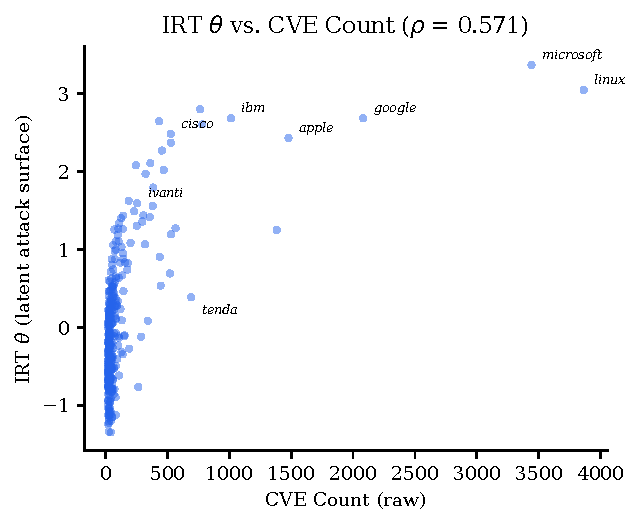
\includegraphics[width=0.65\linewidth]{figures/fig1_theta_vs_count.pdf}
\caption{IRT $\theta$ diverges from raw CVE count ($\rho = 0.571$). Vendors with broad CWE coverage rank higher than those with many CVEs concentrated in few categories.}
\label{fig:theta_count}
\end{figure}

\subsection{Temporal Cross-Validation}

Using 187 common vendors and 145 common CWEs across 2023 and 2024 (Table~\ref{tab:temporal}; Figure~\ref{fig:temporal}):

\begin{table}[H]
\centering
\caption{Temporal stability of IRT parameters (2023 $\to$ 2024).}
\label{tab:temporal}
\small
\begin{tabular}{@{}lcc@{}}
\toprule
Parameter & $\rho$ & 95\% Bootstrap CI \\
\midrule
IRT $\theta$ (vendor) & 0.763 & $[0.673, 0.835]$ \\
Naive average & 0.759 & $[0.670, 0.830]$ \\
IRT $b$ (CWE) & \textbf{0.889} & $[0.836, 0.927]$ \\
\bottomrule
\end{tabular}
\end{table}

\begin{figure}[H]
\centering
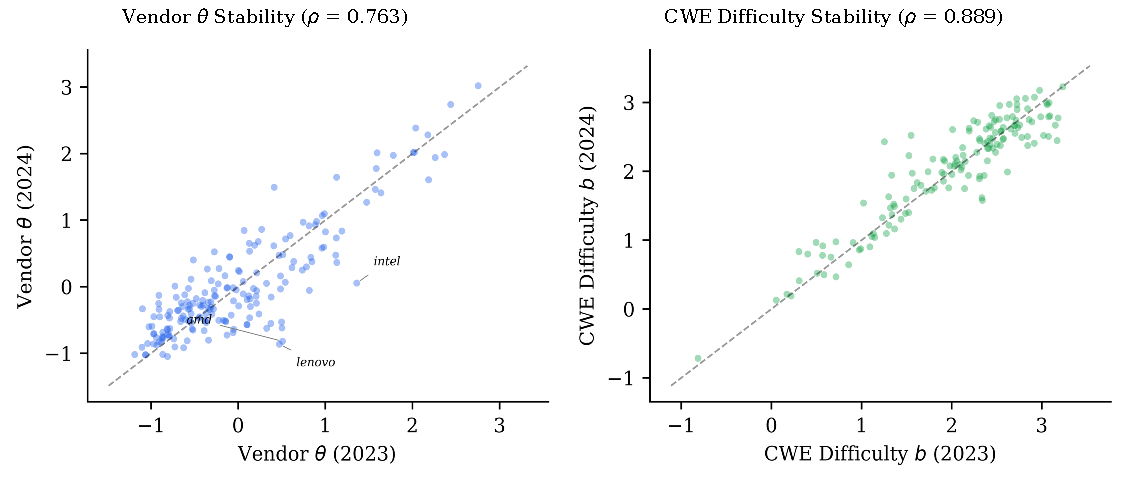
\includegraphics[width=0.85\linewidth]{figures/fig3_temporal_stability.pdf}
\caption{Temporal stability of IRT parameters. Left: Vendor $\theta$ across years ($\rho = 0.763$). The largest absolute year-to-year $\theta$ shifts are annotated; labels indicate vendors with the largest normalized changes between 2023 and 2024. Right: CWE incidence difficulty $b$ is highly stable ($\rho = 0.889$). Note: since 2023 and 2024 models are fitted independently, absolute $\Delta\theta$ values are not directly comparable without scale equating; Spearman~$\rho$ is rank-based and unaffected.}
\label{fig:temporal}
\end{figure}

\subsection{LLTM Feature Decomposition}

\begin{table}[H]
\centering
\caption{LLTM results: predicting IRT difficulty $b$ from observable features.}
\label{tab:lltm}
\small
\begin{tabular}{@{}lccc@{}}
\toprule
Feature Set & $\rho$ & $R^2$ & 95\% CI on $\rho$ \\
\midrule
CVSS only (23 features) & 0.289 & 0.120 & $[0.121, 0.433]$ \\
CVSS + CWE hierarchy (28) & \textbf{0.405} & \textbf{0.210} & $[0.251, 0.537]$ \\
CWE hierarchy only (5) & 0.254 & 0.068 & --- \\
\bottomrule
\end{tabular}
\end{table}

CVSS base metrics explain only 12\% of CWE difficulty variance (Table~\ref{tab:lltm}).
Adding CWE abstraction-level features increases $R^2$ to 21\%.
The remaining 79\% reflects factors not encoded in either system: ecosystem prevalence, tooling coverage, and developer awareness.
Figure~\ref{fig:lltm} shows the top LLTM feature weights.
The dominant feature is average CVSS score ($\eta = -4.09$): higher-CVSS CWEs tend to be \textit{more common} across vendors, not rarer.

\begin{figure}[H]
\centering
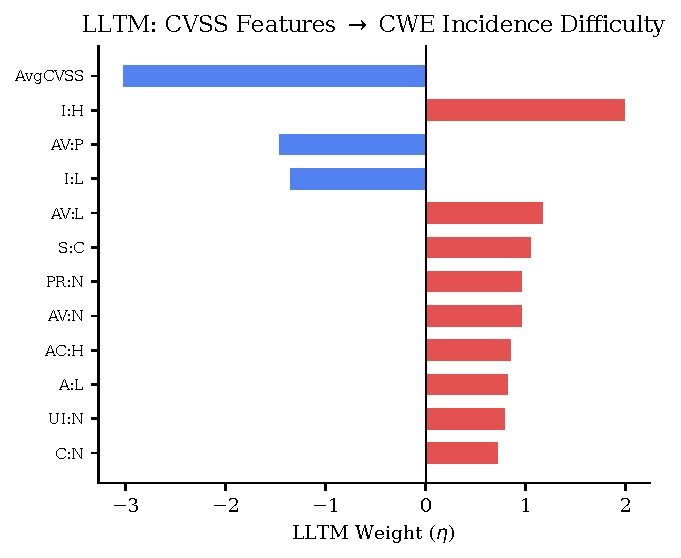
\includegraphics[width=0.6\linewidth]{figures/fig4_lltm_weights.pdf}
\caption{LLTM feature weights ($\eta$). Red bars indicate features associated with higher CWE difficulty (rarer); blue bars with lower difficulty (more common).}
\label{fig:lltm}
\end{figure}

\subsection{Triple Exploitation-Signal Cross-Validation}

IRT difficulty~$b$ is cross-validated against three independent exploitation-signal datasets (Table~\ref{tab:triple}; Figure~\ref{fig:exploitation}).
Negative correlations confirm that \textbf{common CWE types (lower $b$) are more exploited}.

\begin{table}[H]
\centering
\caption{IRT difficulty $b$ vs.\ exploitation rates (CWE-level, $n = 169$).}
\label{tab:triple}
\small
\begin{tabular}{@{}lccl@{}}
\toprule
Exploitation Signal & $\rho$ ($b \leftrightarrow$ rate) & $p$-value & 95\% CI \\
\midrule
CISA KEV rate & $-0.224$ & 0.003 & $[-0.383, -0.069]$ \\
ExploitDB rate & $\mathbf{-0.362}$ & $1.3 \times 10^{-6}$ & $[-0.506, -0.204]$ \\
EPSS mean & $-0.097$ & 0.211 & $[-0.252, +0.057]$ \\
\midrule
\multicolumn{4}{@{}l}{\textit{Vendor-level validation ($n = 110$ vendors with $\geq 1$ KEV or ExploitDB entry):}} \\
$\theta \leftrightarrow$ KEV count & $+0.478$ & $< 10^{-6}$ & $[+0.310, +0.622]$ \\
\bottomrule
\end{tabular}
\end{table}

\begin{figure}[H]
\centering
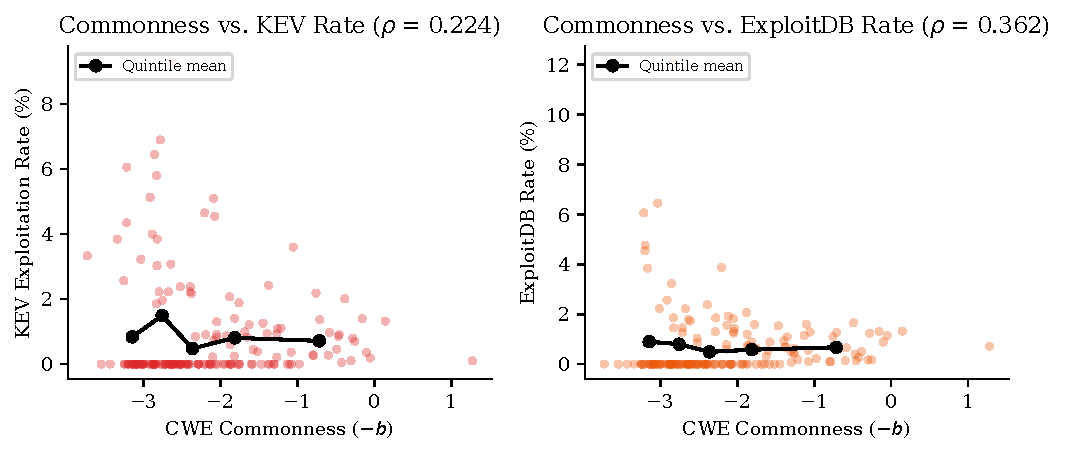
\includegraphics[width=0.85\linewidth]{figures/fig2_difficulty_vs_exploitation.pdf}
\caption{CWE commonness ($-b$) vs.\ exploitation rates. More common CWE types (higher $-b$) have higher exploitation rates in both KEV ($\rho = 0.224$, $p = 0.003$) and ExploitDB ($\rho = 0.362$, $p = 1.3 \times 10^{-6}$). The relationship is statistically significant but modest at the quintile level, consistent with exploitation targeting prevalent weakness categories. Visual quintile bins are descriptive; reported $\rho$ values are Spearman rank-based.}
\label{fig:exploitation}
\end{figure}

The KEV $\leftrightarrow$ EPSS inter-correlation is $\rho = 0.499$; KEV $\leftrightarrow$ ExploitDB is $\rho = 0.263$; EPSS $\leftrightarrow$ ExploitDB is $\rho = 0.364$.
The three exploitation-signal datasets capture partially overlapping but distinct dimensions of exploitation risk.
We use current EPSS scores as a contemporaneous exploitation-likelihood signal, not as a historical pre-disclosure prediction benchmark.
Vendor-level KEV matching uses lowercased CPE vendor strings against KEV \texttt{vendorProject} fields; this is approximate and may miss aliases or vendor renamings.

\subsection{Ransomware Signal}

CWEs linked to known ransomware campaigns ($n = 32$) have significantly lower IRT difficulty than non-ransomware CWEs ($n = 137$; Figure~\ref{fig:ransomware}).
Ransomware-linked CWEs are defined from KEV entries marked \texttt{Known} for ransomware use, intersected with the 2023--2024 NVD CVE subset used in this study:

\begin{table}[H]
\centering
\caption{Ransomware vs.\ non-ransomware CWE parameters.}
\label{tab:ransomware}
\small
\begin{tabular}{@{}lccc@{}}
\toprule
& Ransomware & Non-ransomware & Mann-Whitney $p$ \\
\midrule
Mean $b$ (difficulty) & $+1.19$ & $+2.38$ & $< 10^{-9}$ \\
Mean $a$ (discrimination) & $1.22$ & $1.31$ & $5 \times 10^{-4}$ \\
\bottomrule
\end{tabular}
\end{table}

\begin{figure}[H]
\centering
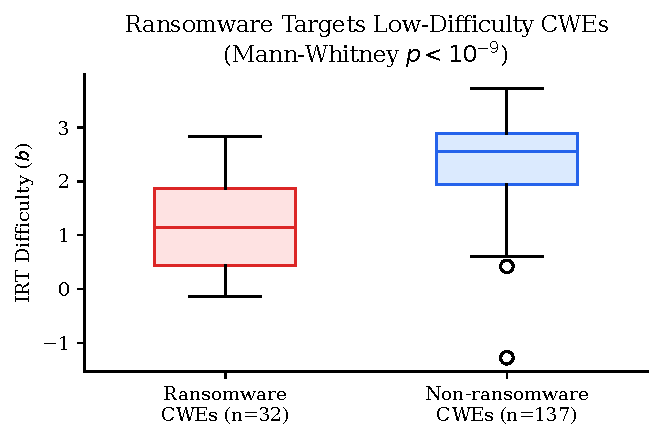
\includegraphics[width=0.55\linewidth]{figures/fig5_ransomware.pdf}
\caption{Ransomware-linked CWEs have significantly lower IRT difficulty, indicating that ransomware operators target common, broadly-prevalent weakness types.}
\label{fig:ransomware}
\end{figure}

This pattern is consistent with official MITRE data: CWE-79 ranked \#1 in the 2024 CWE Top~25 Most Dangerous Software Weaknesses, yet it does not appear in MITRE's 2024 Top~10 KEV Weaknesses list~\citep{cwetop25}.

\subsection{PCR Prioritization}

PCR generates vendor-specific CWE prioritization using the IRT information function.
Validated against KEV exploitation rates:

\begin{table}[H]
\centering
\caption{PCR prioritization lift over random baseline.}
\label{tab:pcr}
\small
\begin{tabular}{@{}lcrrc@{}}
\toprule
Vendor & $\theta$ & PCR KEV Rate & Random & Lift \\
\midrule
google & $+2.68$ & 0.0179 & 0.0079 & $\mathbf{2.28\times}$ \\
ibm & $+2.68$ & 0.0179 & 0.0088 & $\mathbf{2.05\times}$ \\
fedoraproject & $+2.80$ & 0.0103 & 0.0088 & $1.16\times$ \\
linux & $+3.05$ & 0.0103 & 0.0091 & $1.13\times$ \\
microsoft & $+3.37$ & 0.0067 & 0.0085 & $0.78\times$ \\
\bottomrule
\end{tabular}
\end{table}

Among the top-5-$\theta$ vendors evaluated, PCR achieves $2\times$ lift for google and ibm, where the information function is most discriminating.
For extreme-$\theta$ vendors (Microsoft), PCR prioritizes the rarest CWEs, producing a trade-off between coverage breadth and exploitation likelihood.

\section{Discussion}

\paragraph{What IRT Adds.}
IRT transforms the vendor$\times$CWE incidence profile into two interpretable latent traits: vendor breadth $\theta$ and CWE incidence difficulty $b$.
A vendor with $\theta = +2.5$ has a broad attack surface spanning approximately 60\% of CWE categories, regardless of whether it has 500 or 5,000 individual CVEs.
CWE difficulty $b = +3.0$ means a weakness type present in only approximately 3\% of vendors.

\paragraph{Limitations.}
The vendor$\times$CWE matrix is fully observed: every cell represents an observed public-disclosure outcome within the NVD 2023--2024 window, not an intentionally missing test result.
This differs from the natural missingness in educational testing and drug response, where items genuinely go untested.
Consequently, the IRT ranking-stability advantage under structured missing data---demonstrated in the EFSL paper~\citep{kang2026efsl}---does not directly transfer to this formulation.
The proper cybersecurity analog would be MITRE ATT\&CK Evaluation data, where vendors self-select which evaluations to participate in, creating structured missingness.

Our LLTM-inspired decomposition fits IRT first, then regresses the estimated $b$ parameters on CVSS features post hoc, rather than jointly estimating feature weights within the IRT likelihood.
This is a common practical simplification, but means the $R^2$ values should be interpreted as descriptive, not as a formal LLTM model fit.

Because the model depends on NVD CWE assignments, missing or delayed CWE mapping in NVD records---particularly for 2024 CVEs during the NVD enrichment slowdown---may bias the observed vendor$\times$CWE incidence matrix.
MITRE ATT\&CK v19 is included as contextual metadata for CWE-to-technique mapping, not as a core analytic input to the IRT model.

The $R^2$ of 0.21 indicates that CVSS features are structurally incomplete for explaining CWE difficulty.
This is a domain finding: what makes a CWE type rare or common is driven by software ecosystem factors that no severity scoring system captures.

\section{Conclusion}

We demonstrate that psychometric methods---IRT, LLTM, and PCR---reveal interpretable latent structure in the cybersecurity vulnerability landscape that existing scoring systems miss.
CWE difficulty is temporally stable ($\rho = 0.889$), significantly associated with two of three exploitation-signal datasets (KEV and ExploitDB; EPSS not significant, $\rho = -0.097$, $p = 0.211$), and explains ransomware targeting patterns ($p < 10^{-9}$).
CVSS, designed for individual vulnerability severity, alone captures 12\% (in-sample $R^2$; 21\% with CWE hierarchy features added) of the variance in what makes entire weakness categories rare or common.
PCR provides vendor-specific prioritization with positive lift for four of the top-5-$\theta$ vendors, while revealing underperformance for the highest-$\theta$ vendor where the information function saturates.

\paragraph{Data Availability.}
All data sources are publicly available:
\begin{itemize}\setlength{\itemsep}{0pt}\setlength{\parskip}{0pt}
\item NVD: \texttt{github.com/fkie-cad/nvd-json-data-feeds} (community reconstruction of NVD JSON~2.0 feeds, synchronized with the official NVD API; not endorsed by NIST)
\item CISA KEV: \texttt{github.com/cisagov/kev-data}
\item EPSS: \texttt{first.org/epss/api}
\item ExploitDB: \texttt{gitlab.com/exploit-database/exploitdb}
\item CWE: \texttt{cwe.mitre.org/data/csv}
\item ATT\&CK: \texttt{github.com/mitre-attack/attack-stix-data}
\end{itemize}

\bibliographystyle{plainnat}
\begin{thebibliography}{99}

\bibitem[Allodi and Massacci(2014)]{allodi2014}
L.~Allodi and F.~Massacci.
\newblock Comparing vulnerability severity and exploits using case-control studies.
\newblock \emph{ACM Transactions on Information and System Security}, 17(1):Article~1, 2014.

\bibitem[CISA(2021)]{bod2201}
CISA.
\newblock Binding Operational Directive 22-01: Reducing the significant risk of known exploited vulnerabilities.
\newblock 2021.

\bibitem[FIRST(2019)]{cvss31}
FIRST.
\newblock Common Vulnerability Scoring System v3.1 Specification.
\newblock \url{https://www.first.org/cvss/v3.1/specification-document}, 2019.

\bibitem[Fischer(1973)]{fischer1973}
G.~H. Fischer.
\newblock The linear logistic test model as an instrument in educational research.
\newblock \emph{Acta Psychologica}, 37:359--374, 1973.

\bibitem[Jacobs et~al.(2021)]{jacobs2021epss}
J.~Jacobs, S.~Romanosky, B.~Edwards, I.~Adjerid, and M.~Roytman.
\newblock Exploit prediction scoring system (EPSS).
\newblock \emph{Digital Threats: Research and Practice}, 2(3):Article~20, 2021.

\bibitem[Kang(2026)]{kang2026efsl}
J.~M.~Kang.
\newblock The Scaling Law of Evaluation Failure.
\newblock \emph{arXiv:2605.11205}, 2026.

\bibitem[Lord and Novick(1968)]{lord1968}
F.~M.~Lord and M.~R.~Novick.
\newblock \emph{Statistical Theories of Mental Test Scores}.
\newblock Addison-Wesley, 1968.


\bibitem[NIST(2026)]{nist2026}
NIST.
\newblock NVD Program Transition to risk-based triage.
\newblock \url{https://www.nist.gov/news-events/news/2026/04/nist-updates-nvd-operations-address-record-cve-growth}, 2026.

\bibitem[Poulsen et~al.(2021)]{poulsen2021cci}
S.~Poulsen, G.~L.~Herman, P.~A.~H.~Peterson, et~al.
\newblock Psychometric evaluation of the Cybersecurity Concept Inventory.
\newblock \emph{ACM Transactions on Computing Education}, 22(1):Article~6, 2021.

\bibitem[MITRE(2024b)]{cwetop25}
MITRE.
\newblock 2024 CWE Top~25 Most Dangerous Software Weaknesses and Top~10 KEV Weaknesses.
\newblock \url{https://cwe.mitre.org/top25/archive/2024/2024_top25_list.html} and \url{https://cwe.mitre.org/top25/archive/2024/2024_kev_list.html}, 2024.

\bibitem[Koscinski et~al.(2025)]{conflicting2025}
J.~Koscinski et~al.
\newblock Conflicting scores, confusing signals: An empirical study of vulnerability scoring systems.
\newblock In \emph{ACM CCS}, 2025.

\bibitem[BitSight(2024)]{bitsight2024}
BitSight.
\newblock Evaluating dependence on NVD.
\newblock Blog, \url{https://www.bitsight.com/blog/evaluating-dependence-on-nvd}, June 2024.

\bibitem[Suciu et~al.(2017)]{suciu2017latent}
O.~Suciu et~al.
\newblock Latent feature vulnerability ranking of CVSS vectors.
\newblock In \emph{SummerSim}, 2017.

\end{thebibliography}

\end{document}
